% !TEX root = ./../main.tex
\chapter{Model of biological membrane and charged protected gold NP}

\section{NanoParticle model}

% gold core --> Thyiol passivated --> ligands
%Ligand Composition: Patched (1:1), Random (1:1) (1:2)
%Different level of hydrophobicity
%Different ligand charge: anionic/cationic NP

\subsection{Passivated gold core}
\acp{NP} with gold core can be stabilized by thiols, which stably bind to the Au surface via Au--S bonds. Thiolated Au\acp{NP} are air stable, electrochemically stable and thermally stable compounds []. Our Au\ac{NP} is built on the {Au$_{144}$(SR)$_{60}$}. The gold core is composed by $144$ atoms which displays icosahedral symmetry and it is made of three bulk shell with $12$, $42$ and $60$ atoms, respectively. A surface shell of $30$ atoms completes the gold cluster structure. Then $60$ sulphur atoms, which blind the aliphatic chains (R) to the gold core, are bounded to the gold atoms on the surface through the typical bond structure RS--Au--SR. The shell construction is shown in figure~(\ref{fig:goldShell}).
\begin{figure}[!ht]
	\centering
	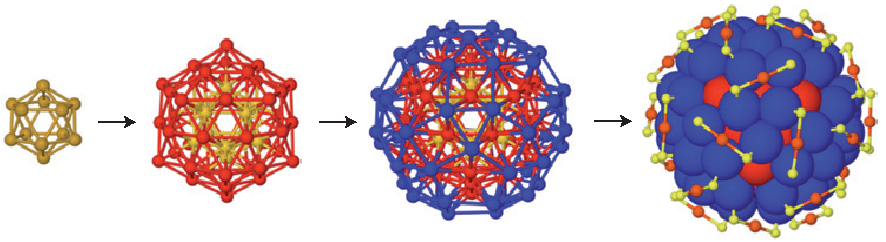
\includegraphics[width=0.9\textwidth]{./img/goldShell}
	\caption{First three frame: the concentric $12$--(yellow), $42$--(red) and $60$--(blue) atom gold internal shell, surrounded (last frame) by $30$ gold (red small) and $60$ sulphur (yellow small) surface atoms. The R chains is not show. Taken from \cite{corePassivated}.}
	\label{fig:goldShell}
\end{figure}

The resulting diameter of the gold core is about $2$~nm. When passivated by thiols, its overall size depends on the length of the aliphatic chains bound to the sulphur atoms. The monolayer--protected Au\ac{NP} we will consider have a total diameter of about $4$~nm.

Despite the computational cost associated to atomistically describe the gold cluster, all gold atoms are taken into account in order to allow us future studies on heating effect on lipid bilayer. Thus the bonds between gold atoms are allowed to vibrate. As we have seen in a previous section, a many--body potential should be used. Instead, as we are interested in the vibrational modes of the core atoms, Federica Simonelli in her thesis work, found that a more efficient way is to use an elastic network associated the potential energy
\begin{equation*}
	U = \frac{1}{2}\sum_i \sum_{j\ne i}k_{ij}(r_{ij} - r_{ij}^0)^2
\end{equation*}
where $r_{ij}$ is the distance and $k_{ij}$ is the bond constant for $i-j$ atom pair. The bond constants were assigned so as to reproduce the vibrational spectrum of the gold core as provided by the many--body Gupta potential. The constant were assigned to $k = 32500$~kJ/(mol\,nm$^2$) for surface atoms and $k = 11000$~kJ/(mol\,nm$^2$) for bulk atoms. While the equilibrium distances were derived from []. In figure~(\ref{fig:goldNetwork}) the gold elastic network is shown.
\begin{SCfigure}
	\centering
	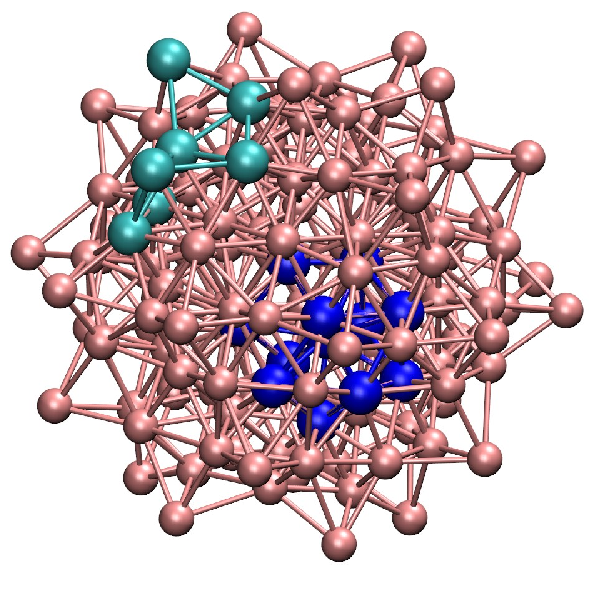
\includegraphics[width=0.4\textwidth]{./img/goldNetwork}
	\caption{Elastic network, represented by the stick bond, among gold atoms (pink). In cyan a surface atoms and its neighbors. In blue a group of bulk atoms and its neighbors. Taken from \cite{simonelliThesis}.}
	\label{fig:goldNetwork}
\end{SCfigure}

An elastic network with bond constant of $1250$~kJ/(mol\,nm$^2$) was also used to model sulphur atoms on the surface of the \ac{NP} cluster with a cutoff distance of $0.55$~nm to select the sulphur neighbor atoms. The interaction between a sulphur atom and its nearest gold atoms was modeled through a harmonic potential with a bond constant of $32500$~kJ/(mol\,nm$^2$) and equilibrium distances given by []. In order to prevent the penetration of the sulphur atoms into gold core, a repulsive potential of the form $C/r^{-12}$ where $C = 0.92953\cdot 10^-6$~kJ\,nm$^{12}$/mol models the non--bonded interaction between gold and sulphur atoms which are not involved in any of the previous bonds. In figure~() sulphur passivated \ac{NP} gold cluster with the complete elastic network is shown.

% some information about gold core: dimensions, number of atoms, model used, elastic network, shel construction

\subsection{Functionalizing ligands}

%\subsection{OT ligands}
\paragraph{\textbf{OT Ligands}} They are completely hydrophobic compounds made by seven \ac{CH2} groups and one \ac{CH3} terminal group. Two \martini beds of type C$_1$ model the eight carbon atoms of the \ac{OT} backbone and their hydrogen atoms. The chemical structure and the resulting \ac{CG} \martini model is shown in figure~(). The first bead of each \ac{OT} ligands is bound to a sulphur atom via a harmonic potential with a bond constant of $1250$~kJ/(mol\,nm$^2$) and equilibrium length of $0.47$~nm. The second bead is connected to the first by same bond potential. An angle potential as in equation~\eqref{eq:martiniAngle} is used among the three particles. Parameters are fixed in accordance with the standard \martini ones (see section~\ref{sec:martiniPotential}). Moreover a purely repulsion potential, as described in the previous section, is used between C$_1$ beads and gold and sulfur atoms to prevent the co--penetration.

%\subsubsection{MUS ligands} %Anionic an the cationic???
\paragraph{\textbf{MUS Ligands}} They are charged compounds made of eleven \ac{CH2} groups and a charged terminal \ac{SO4-} group. The charged terminal group make them partially hydrophilic. Three \martini beads of type C$_1$ model the hydrophobic chain even if one of them groups three carbon atoms instead of four. The charged group is modeled as a Q$_\text{da}$ beads with a charge of $-\mathsf{e}$. The chemical structure and the resulting \ac{CG} \martini model is shown in figure~(). Even in this case the first bead of a \ac{MUS} ligand is bounded to the sulphur atom through a harmonic potential with the same parameter: bond constant of $1250$~kJ/(mol\,nm$^2$) and equilibrium length of $0.47$~nm. The same potential is used to bind all other beads to the previous one. An angle potential as in equation~\eqref{eq:martiniAngle} is used among the sulfur atom, the first C$_1$ and second C$_1$, among the first, the second and the third C$_1$ beads and so on for all four beads. Parameters are fixed in accordance with the standard \martini ones (see section~\ref{sec:martiniPotential}). As in the \ac{OT} ligand model, a purely repulsion potential, as described in the previous section, is used between C$_1$ beads and gold and sulfur atoms to prevent the co--penetration. The same applies between Q$_\text{da}$ beads and gold and sulfur atoms.

\section{Model biological membrane}

\subsection{Real membrane}

\subsection{MARTINI model}

\section{NP--Membrane interaction}

\subsection{Three--stage process}

\subsection{Preliminary free energy calculations}